%!TEX root = ../dokumentation.tex

\chapter{Technische Grundlagen}

\section{Verwendete Bibliotheken}

\section{Architektur}

Um die Ziele der Erweiterbarkeit, Wartbarkeit und einfachen Verständlichkeit zu erfüllen, ist eine modulare Aufbauweise des Projektes von Nöten. Die auf diesen Prinzipien beruhende Architektur wird im folgenden Kapitel beschrieben.

Zunächst wurde das Programm der Aufgaben entsprechend in einzelne Klassen unterteilt, die verschiedene Aufgaben zugewiesen bekommen haben. Diese Aufteilung kann Figur 3.2.1 entnommen werden.

\begin{figure}[h]
\centering
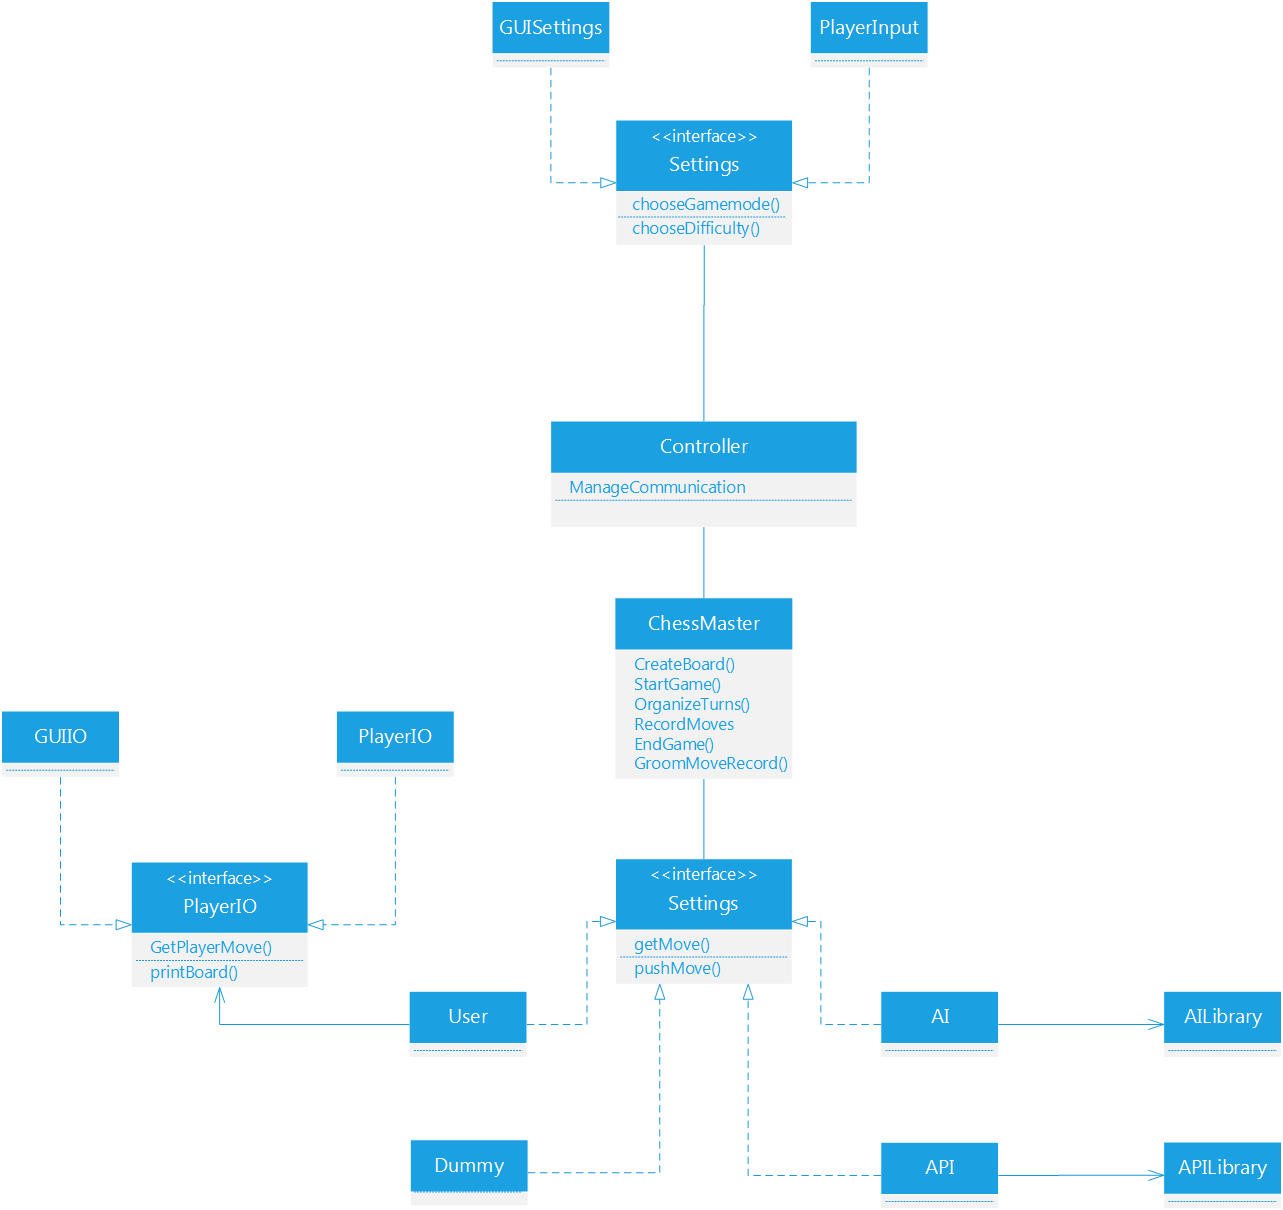
\includegraphics[width=\textwidth*4/5]{images/architecture_class_diagram.png}

\textsuperscript{Figur 3.2.1 Klassendiagramm Architektur ChessAI}
\end{figure}

Als zentrales, Verbindungselement steht zunächst der ``Controlle''. Dieser übernimmt die Abfrage aller Optionen, falls diese nicht beim Start des Programms mit übermittelt werden. Zudem initialisiert der Controller die Spielteilnehmer sowie den ``ChessMaster''. Bei letzterem übergibt der Controller diesem die initialisierten Spielteilnehmer. Die Aufgaben des ``ChessMaster'' wird später genauer beschrieben.

Zur Abfrage der Optionen steht dem Controller eine `Settings' Schnittstelle zur Verfügung. Diese wird für Eingaben des Nutzers einerseits über eine Konsole als auch optional über eine grafische Nutzeroberfläche implementiert. Dabei wird abgefragt, welchen Typ die jeweiligen Spielteilnehmer annehmen sollen und es können zudem zusätzliche Optionen für die einzelnen Spieler definiert werden. Als Beispiel kann für Spieler 1 der Typ ``User'' gewählt werden und für Spieler 2 der Typ ``AI''. Dies ermöglicht ein Spiel des Nutzers gegen die im Rahmen dieser Arbeit entwickelte KI. Für die KI wird darauf folgend noch der Schwierigkeitsgrad abgefragt. Zusätzlich kann für jeden Spieler ein Name festgelegt werden.

Die Aufgaben des ``ChessMaster'' erstrecken sich über die Verwaltung des Schachspiels an sich, das Ansprechen der jeweiligen Spieler zum Ermitteln ihrer Züge sowie dem Durchführen des gewählten Spielzugs auf dem Schachbrett. Zusätzlich speichert es jedes Schachbrett, das sich im Laufe des Spiels ergibt, und fügt diese zur ``board\_history.'' Datei hinzu. Diese speichert alle Schachbretter gemeinsam mit einem numerischen Wert. Dieser gibt Aufschluss über Erfolgsaussichten der jeweiligen Akteure des Spiels. Dazu wird nach jedem Spiel zu dem entsprechenden Eintrag in der Datei eine eins zu dem alten Wert aufaddiert, wenn der Spieler der weißen Figuren das Spiel gewonnen hat und eine eins subtrahiert, wenn der Spieler der schwarzen Figuren das Spiel gewonnen hat. Bei einem Unentschieden bleibt der alte Wert bestehen. Dies hilft der KI bei der Bewertung eines Schachbretts unter zur Hilfenahme von statistischen Werten. 

Dieser spricht die vom Controller erstellten Spieler an. Diese können, wie bereits angedeutet, von verschiedenen Typen sein. Zur Auswahl stehen
\begin{itemize}
\item User - Ein menschlicher Akteur kann Züge über eine Nutzerschnittstelle eingeben
\item AI - Die künstliche Intelligenz versucht den best möglichsten Zug zu berechnen
\item Dummy - Ein zufälliger Zug wird ausgewählt
\item (Optional) API - Ein Zug wird über eine Schnittstelle zu einer Online Schachplattform, auf der menschliche sowie künstliche Spieler teilnehmen dürfen, bestimmt
\end{itemize}

Dazu existiert eine ``Player'' Schnittstelle, die für jeden dieser Spieler implementiert werden muss.

Die ``User'' Implementation greift dabei zur Ermittlung des Zuges auf eine ``PlayerIO'' Schnittstelle zurück. Diese wiederum kann - ähnlich zur ``SettingsUI'' Schnittstelle - sowohl für Eingaben über eine Konsole als auch für Eingaben über eine grafische Nutzeroberfläche implementiert werden.

Die ``AI'' sowie die ``API'' Implementation greifen für die Ermittlungen ihrer Züge nochmals auf eigens erstellte Bibliotheken zurück, die elementare Funktionen erhalten.

Der genaue Ablauf der Ermittlung der Züge sowie der andere Operationen des Programmes werden in Kapitel XY.ZY näher erläutert.

In Figur 3.2.2 ist der sequenteille Ablauf der Funktionsaufrufe erkennbar.

\begin{figure}[h]
\centering
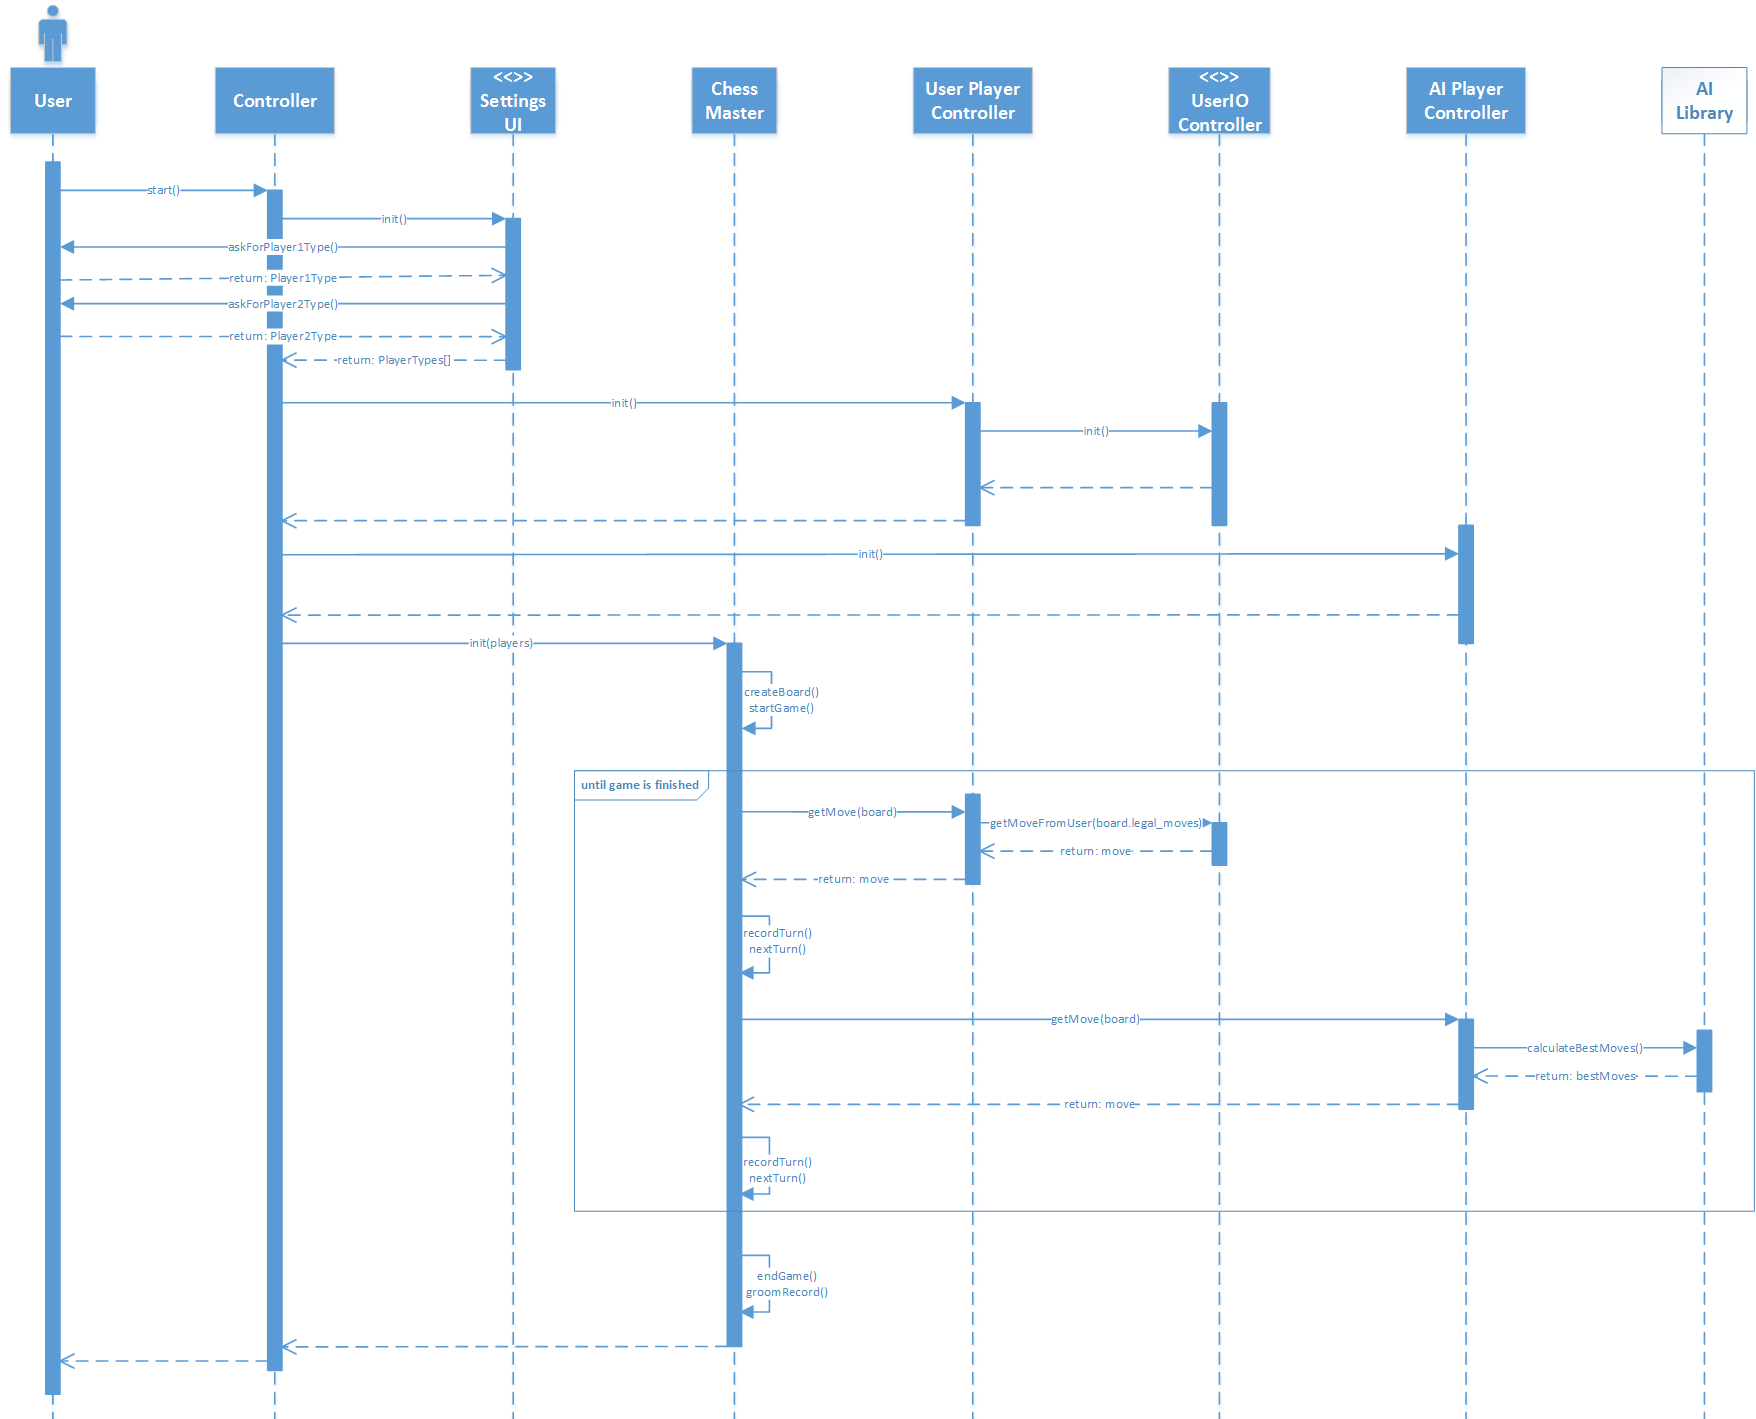
\includegraphics[width=\textwidth]{images/architecture_sequence_diagram.png}

\textsuperscript{Figur 3.2.2 Sequenzdiganagramm Architektur ChessAI}
\end{figure}

Dabei wird zunächst über die ``Settings'' Schnittstelle nach den Spielertypen sowie Namen gefragt. initialisiert der ``Controller'' die Spieler, in diesem Fall einerseits den ``User'', der wiederum die ``UserIO'' Schnittstelle implementiert, und außerdem den ``AI'' Player. 

Darauffolgend spricht der ``Controller'' den ``ChessMaster'' an. Dieser startet nun das Spiel und fragt solange wie das Spiel nicht vorbei ist immer abwechselnd erst zu Spieler 1 - dem Nutzer - und dann zu Spieler 2 - der KI - nach dem nächstne Zug. Dabei übergibt der ``ChessMaster'' stets das aktuelle Schachbrett. Der Nutzer ermittelt den durchzuführenden Zug über eine Abfrage an den Nutzer über die entsprechende Schnittstelle, der ``AI'' Spieler, indem dieser Funktionen aus der entsprechenden Bibliothek zur Hilfe nimmt.

Nach jedem Zug fügt der ``ChessMaster'' diesen zum Schachbrett hinzu und speichert dieses in einen Spielverlauf. Nach Ende des Spiels wird dieser in das ``board\_history.csv'' eingepflegt wie weiter oben bei der Beschreibung der Klasse bereits erläutert.

Abschließend beendet der ``ChessMaster'' das Spiel, wenn keine Revance gewünscht ist, und so wird auch das Programm im Anschluss daran geschlossen.


%TODO: CSV zur Architektur hinzufügen; Funktionsnamen python way
